% !TeX root = ../main.tex

\section{Background and Motivation}\label{sec:background}


\subsection{Regulatory Requirement for Data Security}

\begin{figure*}[!t]
    \centering
    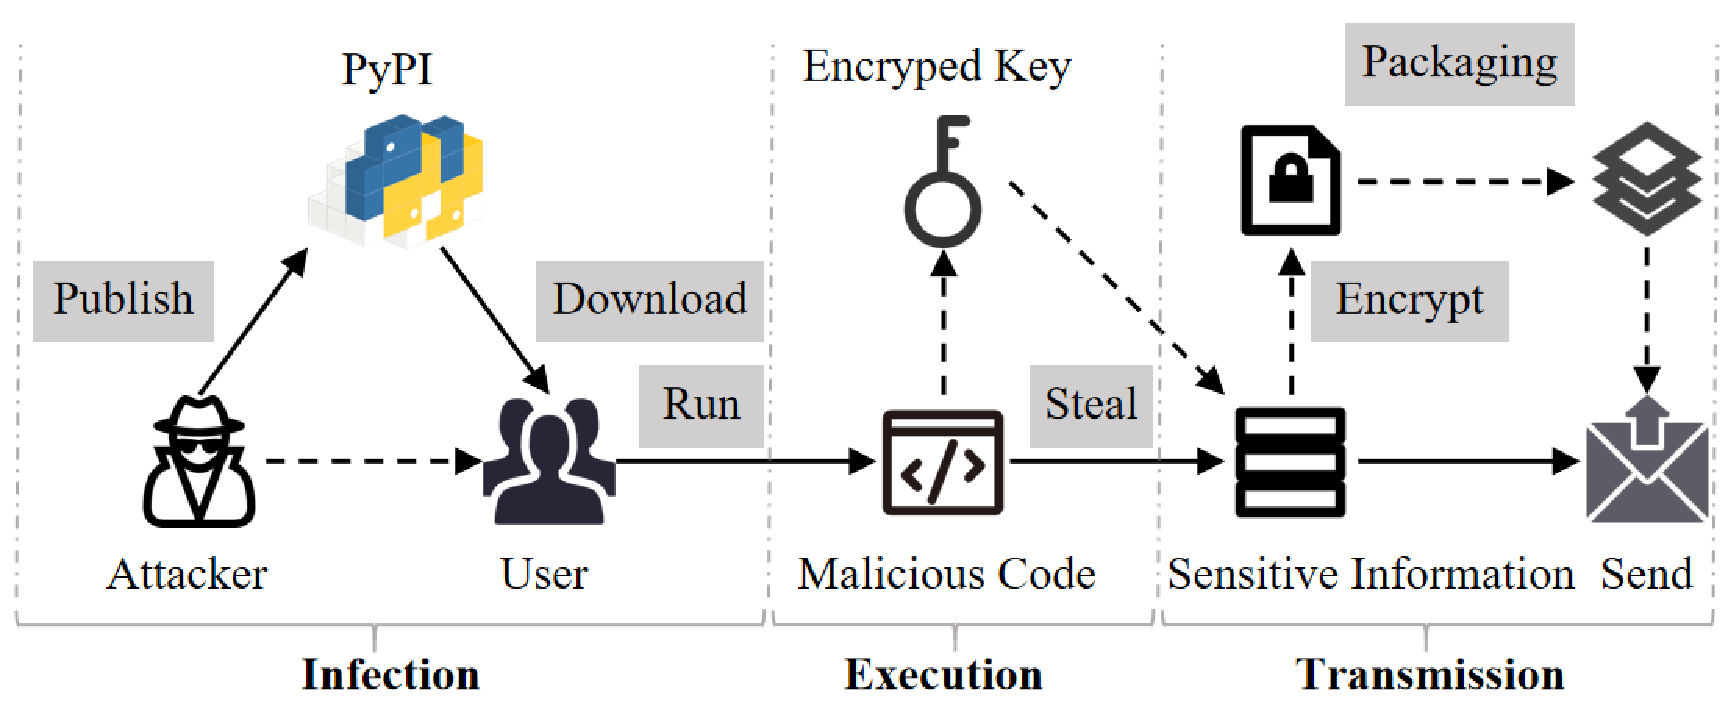
\includegraphics[width=0.8\textwidth]{fig/execution_process.pdf}
    \vspace{-10pt}
    \caption{Typical Actions for Malicious Data Exfiltration Packages}
    \label{fig:Execution_Process}
\end{figure*}

The significance of data has been widely recognized, as breaches in data security can cause significant harm to individuals, organizations, and critical infrastructure. Consequently, protecting data from unlawful use has become a priority, addressed not only through governmental advocacy but also through the establishment of legal frameworks. One of the most influential regulatory frameworks is the European Union's General Data Protection Regulation (GDPR)~\cite{gdpr} taking effective in 2018, which requires \todo{data controllers and processors} to implement robust measures to safeguard personal data. In the United States, the Computer Fraud and Abuse Act (CFAA)~\cite{CFAA1986} prohibits unauthorized access to computer systems and criminalizes the transmission or theft of data. It serves as a primary legal tool for prosecuting cybercriminals involved in data exfiltration activities, including both external attackers and malicious insiders. \todo{China?} Examples of sector-specific regulations include the Health Insurance Portability and Accountability Act (HIPAA)~\cite{HIPAA1996}, which addresses data exfiltration risks within the healthcare sector. Generally, governments have  enacted strict regulations to safeguard data, which not only deter cybercriminals but also prompt potential victims to be more vigilant about data security.

\subsection{Malicious Data Exfiltration Packages}

We provide the definition of malicious data exfiltration packages and describe their typical actions.

\textbf{Definition of data exfiltration packages.} We provide the criteria for determining malicious data exfiltration packages: 

\textbf{\textit{Malicious data exfiltration packages access and transfer users'~sensitive information without their knowledge or consent.}}
Specifically, we use two indicators to determine whether a malicious package is a data exfiltration package:
\begin{itemize}
    \item \textit{Obtaining sensitive information}: A package uses system collection or environment collection to obtain sensitive information from a computer.
    \item \textit{Transmitting sensitive information}: A package sends the obtained information to a certain URL.
\end{itemize}



Fig. \ref{fig:Execution_Process} presents the typical actions for malicious data exfiltration packages. 
First, attackers publish malicious packages on PyPI, 
which were then downloaded on the local environment of 
and after users download and run them, some packages will decrypt authentication information to obtain Encryped\_keys. Afterwards, malicious code will use the Encryped\_key to steal sensitive information through system functions or other means. After obtaining the information, some packages will encrypt and package it, finally send it to URLs controlled by attackers, exfiltrating sensitive information.


\begin{itemize}
    \item \textbf{Infection.} Typosquatting\todo{CITE HERE} is one of the most common infection vectors on PyPI, where malicious packages are given names that closely resemble those of legitimate libraries (e.g., request vs. requests), tricking developers into accidental installation. Besides, \todo{in the case of ctx}, attackers also leverage a typical technique of a repository account takeover where the attacker tries to find a popular repository owned by an email whose domain has expired. \todo{Then, the attacker could re-register the same domain and re-create maintainers' email to obtain the control of the repository.}
    \item \textbf{Execution.} Once a malicious PyPI package is shipped , either directly or as a transitive dependency, it typically employs stealthy execution methods to initiate its payload while minimizing user suspicion. In the context of PyPI-distributed malware, one common technique involves abusing Python's package installation hooks. Attackers may inject code into the setup.py script so that it executes automatically during the pip install process, triggering the exfiltration logic before the package is even imported by the user~\cite{guo2023empirical}. Another widely used technique is the inclusion of malicious code in the \_init\_.py file, ensuring that the payload is executed immediately upon importing the package. The malware will execute code inside the file that's automatically executed when the module is imported.
    \item \textbf{Transmission.} The execution process of a data exfiltration package inevitably includes obtaining and transmitting information. And these two steps will give rise to other operations, such as decrypting authentication information, encrypting and packaging information.
\end{itemize}


After successfully exfiltrating data from compromised systems, attackers can employ various strategies to monetize the stolen information. These profit mechanisms often depend on the type and sensitivity of the data.
One of the most straightforward strategies is selling exfiltrated credentials and tokens on darknet marketplaces. Cloud service keys, API tokens, and login credentials, especially those associated with high-privilege accounts, are in high demand, as they can be reused for lateral attacks, privilege escalation, or resale to third parties. Attackers may also aggregate these credentials into searchable databases, increasing their market value.~\cite{DarkOwl2022}
In some scenarios, attackers may leverage the exfiltration to deploy secondary payloads, such as ransomware or cryptocurrency miners, especially if the exfiltrated data suggests the host is part of a high-value corporate network. This hybrid model enables both short-term like crypto mining and long-term like ransomware monetization paths.~\cite{GoogleCloud2021}.

% In recent years, attackers have increasingly leveraged open source software ecosystems such as the PyPI to distribute malicious data exfiltration packages. This tactic forms part of a broader software supply chain attack, wherein attackers upload seemingly benign Python libraries. Once these packages are installed, they may silently initiate data collection and exfiltration routines.
% After that, the attacker owns the repository and is able to make desired changes (e.g., embed a malicious code in a release).~\cite{CrowdStrike2024}


\subsection{Motivation}
Despite the growing awareness of software supply chain attacks, malicious data exfiltration packages on open-source platforms like PyPI remain a largely underexplored threat. This lack of targeted research creates blind spots in both academic understanding and practical defense mechanisms.

Our motivation for designing RQ1 is to understand how prevalent data exfiltration activities have become. Analyzing prevalence helps reveal the commonality and severity of data stealing as a threat.

The motivation for RQ2, RQ3, and RQ4 is to gain a deeper understanding of the technical and strategic characteristics of data exfiltration packages, with the goal of supporting more precise cybersecurity defenses. At present, detection tools for malicious packages, such as CEREBRO, MPHunter, and AMALFI, are primarily developed based on the analysis of malicious behaviors, their effectiveness heavily depends on a clear understanding of the behavioral features commonly exhibited by malicious packages. Therefore, it's necessary to examine the typical attack patterns data exfiltration packages employ (RQ2), the disguise techniques used to evade detection (RQ3), and the specific objectives they are designed to achieve (RQ4). Such insights are essential for designing detection systems that can identify malicious behavior accurately.

The motivation for RQ5 is to evaluate the effectiveness of existing detection tools and platforms in identifying data exfiltration malicious packages. By examining their current detection rates, this research aims to assess how well these tools perform in real scenarios. Understanding their strengths and limitations is essential for identifying gaps in current defense mechanisms.